
(本文转载自 \href{https://zhuanlan.zhihu.com/c_1005817911142838272}{桃酱的算法笔记},原文戳 \href{https://zhuanlan.zhihu.com/p/41867199}{链接},已获得作者授权)

一直想学 FFT,之前牛客的多小有一道组合数学就用 FFT 写的,而且当时还傻乎乎的用唯一分解定理,但是自己好久没静下心学什么了,而且自己的数学功底又不好,导致一直学不会。看了很多人的博客也没看明白,尤其是原根。在我看了几十篇博客之后终于看懂了。。。所以想写一篇能够让大多数人都看得懂的教程。花费时间 3 天终于写完啦\sout{}\textbackslash{}\textasciitilde{}\textasciitilde{}

另外,本文 FFT 部分的代码实现全部参考 kuangbin 的模板(2018.7 更新)资源地址如下

\url{https://download.csdn.net/download/qq_37136305/10562410}

NTT 部分代码参考 CSDN 上的模板代码附网址,感谢博主!

你搜索这个关键词就已经知道这一是个数学的东西了。只想学会用很简单,但是这远远不够。所以在看这个博客之前应该先学一下  复数  的基本知识。

好了下面进入正文。

\subsection{DFT IDFT FFT 官方定义?}

\begin{QUOTE}{}{}
离散傅里叶变换(Discrete Fourier Transform,缩写为 DFT),是傅里叶变换在时域和频域上都呈离散的形式,将信号的时域采样变换为其 DTFT 的频域采样。



FFT 是一种 DFT 的高效算法,称为快速傅立叶变换(fast Fourier transform)。 ——百度百科
\end{QUOTE}

在百度百科上能找到 DFT 和 FFT 这两个定义。正如定义,FFT 和 DFT 实际上按照结果来看的话是一样的,但是 FFT 比较快的计算 DFT 和IDFT(离散反傅里叶变换)。

快速数论变换 (NTT) 是快速傅里叶变换(FFT)在数论基础上的实现。

是不是有点迷 QAQ?既然是官方定义那肯定不能让你看懂才对嘛~下面我们一一解释~

\subsection{为什么要使用 FFT?}

我们在这里引入一个例子:求多项式乘积的朴素算法。

大家平时求 $f(x)=a_1x^2+b_1x+c_1$ 与 $g(x) = a_2x^2+b_2x+c_2$ 的乘积时候,是怎么进行的呢?

我们令

$$
K(x) = f(x)  \times  g(x) = a_1x^2 \times a_2x^2+a_1x^2 \times b_2x+a_1x^2 \times c_2+b_1x \times b_2x^2+b_1x \times b_2x+b_1x \times c_2+c_1 \times a_2x^2+c_1 \times b_2x+c_1 \times c_2
$$

那么很显然我们进行了 9 次运算,复杂度是 $O(n^2)$ (具体代码实现不再展开)

但是如果数字足够大呢?比如 100000?那朴素算法可太慢啦 (;′⌒),

\subsection{什么是 FFT}

FFT,即为快速傅氏变换,是离散傅氏变换的快速算法,它是根据离散傅氏变换的奇、偶、虚、实等特性,对离散傅立叶变换的算法进行改进获得的。它对傅氏变换的理论并没有新的发现,但是对于在计算机系统或者说数字系统中应用离散傅立叶变换,可以说是进了一大步。——360 百科

如果上一个例子用朴素算法太慢啦!所以我们要用 FFT 进行优化,复杂度会降为 $O(nlogn)$

\subsubsection{多项式的系数表示法与点值表示法}

一个多项式,我们可以怎样来表示呢?

系数表示法就是用一个多项式的各个项系数来表达这个多项式。比如:

$$
f(x) = a_1x^2+b_1x+c_1 \Leftrightarrow f(x) = \{a_1, b_1, c_1\}
$$

点值表示法是把这个多项式看成一个函数,从上面选取 $n+1$ 个点,从而利用这 $n+1$ 个点来唯一的表示这个函数。为什么用 $n+1$ 个点就能唯一的表示这个函数了呢?想一下高斯消元法,两点确定一条直线。再来一个点,能确定这个直线中的另一个参数,那么也就是说 $n+1$ 个点能确定 $n$ 个参数(不考虑倍数点之类的没用点)。如下:

$$
f_1(x) = y_1 = a_0 + a_1x_1+a_2x_1^2+a_3x_1^3+ \cdots + a_nx_1^n
$$

$$
f_2(x) = y_2 = a_0 + a_1x_2+a_2x_2^2+a_3x_2^3+ \cdots + a_nx_2^n
$$

$$
f_3(x) = y_3 = a_0 + a_1x_3+a_2x_3^2+a_3x_3^3+ \cdots + a_nx_3^n
$$

$$
f_4(x) = y_4 = a_0 + a_1x_4+a_2x_4^2+a_3x_4^3+ \cdots + a_nx_4^n
$$

$$
f_5(x) = y_5 = a_0 + a_1x_5+a_2x_5^2+a_3x_5^3+ \cdots + a_nx_5^n
$$

$$
\cdots
$$

$$
f_n(x) = y_n = a_0 + a_1x_m+a_2x_m^2+a_3x_m^3+ \cdots + a_nx_m^n
$$

一个非常通俗易懂的解释:

多项式由系数表示法转为点值表示法的过程,就成为 DFT;

相对地,把一个多项式的点值表示法转化为系数表示法的过程,就是 IDFT。

而 FFT 就是通过取某些特殊的 $x$ 的点值来加速 DFT 和 FFT 的过程。

\subsubsection{复数的引入}

复数分为实数和虚数。实数就是我们日常最常用的有理数和无理数。大家记得我们在开始学平方的时候,老师会说所有数的平方大于等于 $0$ 对不对,那么虚数就引入了。虚数一般用 $i$ 表示,对于虚数 $i$,有 $i=\sqrt{-1}$

。另外,$i$ 对于虚数的意义,与 $1$ 对于实数的意义是一样的。如果我说得不够明确,你可以看下面我引用的百科说明。

\begin{QUOTE}{}{}
在数学中,虚数就是形如 $a+b \times i$ 的数,其中 $a,b$ 是实数,且 $b \neq 0$,$i^2 = - 1$。虚数这个名词是 17 世纪著名数学家笛卡尔创立,因为当时的观念认为这是真实不存在的数字。后来发现虚数 $a+b \times i$ 的实部 $a$ 可对应平面上的横轴,虚部 $b$ 与对应平面上的纵轴,这样虚数 $a+b \times i$ 可与平面内的点 $(a,b)$ 对应。



可以将虚数 $bi$ 添加到实数 $a$ 以形成形式 $a + bi$ 的复数,其中实数 $a$ 和 $b$ 分别被称为复数的实部和虚部。一些作者使用术语纯虚数来表示所谓的虚数,虚数表示具有非零虚部的任何复数。 ——百度百科
\end{QUOTE}

我们用一幅图来表示复数与复平面的关系(图源百度百科)

\begin{figure}[htbp]
\centering
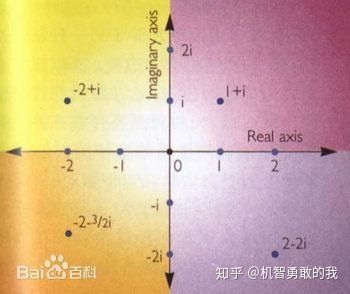
\includegraphics[width=0.7\textwidth]{docs/math/images/fft1.jpg} 
\caption{img}
\end{figure}

其中横坐标是实数轴,纵坐标是虚数轴,这样就可以把每个虚数看为一个向量了,对应的,虚数可以用普通坐标和极坐标 $(r,\theta)$

(其中 $r$ 为虚数长度,$\theta$ 为虚数和实数轴正半轴夹角) 来表示。

接下来思考两个复数相乘是什么意义:

\begin{enumerate}
\item $(a+bi) \times (c+di) = (ac-bd) + (ad+bc)i$
\item 长度相乘,角度相加: $(r_1, \theta_1)  \times  (r_2, \theta_2) = (r_1 \times r_2, \theta_1+\theta_2)$
\end{enumerate}

这么一看的话,我们很容易想到如果两个长度为 $1$ 的不同方向向量相乘,结果向量是不是一个长度依然为 $1$ 的新向量呢?

\subsubsection{单位复根的引入}

我们回到之前的问题:多项式(点值表示法)的乘积。

考虑这样一个问题:

刚刚说到了 DFT 是把多项式从系数表示转到了点值表示(复杂度为 $O(n)$),那么我们把点值相乘之后(选取相应位置,并且复杂度为 $O(n)$),如果能够快速还原成系数表示,是不是就完美解决我们的问题了呢?上述过程如下:

假设我们 DFT 过程对于两个多项式选取的 $x$ 序列相同,那么可以得到

$$
f(x)={(x_0, f(x_0), (x_1, f(x_1)), (x_2, f(x_2), \cdots, (x_n, f(x_n)))}
$$

$$
g(x)={(x_0, g(x_0), (x_1, g(x_1)), (x_2, g(x_2), \cdots, (x_n, g(x_n)))}
$$

如果我们设 $F(x) = f(x) \times g(x0$

那么很容易得到 $F(x)$ 的点值表达式:

$$
F(x) = {(x_0, f(x_0)  \times  g(x_0), (x_1, f(x_1)  \times  g(x_1)), (x_2, f(x_2)  \times  g(x_2), \cdots, (x_n, f(x_n)  \times  g(x_n)))}
$$

但是我们要的是系数表达式,接下来问题变成了从点值回到系数。如果我们带入到高斯消元法的方程组中去,会把复杂度变得非常高。光是计算 $x^i(0 \leq i \leq n)$ 就是 $n$ 项, 这就已经 $O(n^2)$ 了,更别说还要把 $n+1$ 个方程进行消元。。。。。。。。。

这里会不会觉得我们不去计算 $x^i$ 比较好呢?$1$ 和 $-1$ 的幂都很好算,但是也仅仅有两个不够啊,我们至少需要 $n+1$ 个 o(╥﹏╥)o 那怎么办呢!想到我们刚刚学的长度为 $1$ 的虚数了吗?不管怎么乘长度都是 $1$!对就是它!我们需要的是 $\omega^k=1$ 中的 $\omega$,很容易想到 $-i$ 和 $1$ 是符合的。那其他的呢?

\begin{figure}[htbp]
\centering
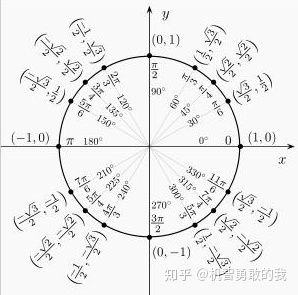
\includegraphics[width=0.7\textwidth]{docs/math/images/fft2.jpg} 
\caption{img}
\end{figure}

现在我们看上图的圆圈。容易发现这是一个单位圆(圆心为原点,半径为 $1$),所有在圆上的复数的长度均为 $1$,也就是说它不管做多少次方 $r$ 永远为 $1$,结果也仅仅角度的变化而已。但是!!!进过旋转总会让角度 $\bmod 360 = 0$ 成立的,也就是结果为 $1$。 我们把符合以上条件的复数成为复根,用 $\omega$ 表示。如果 $\omega^k=1$ 那么我们把$\omega$ 称为 $1$ 的 $k$ 次复根,记作 $\omega_k^n$ (因为符合这个 $k$ 次之后等于 $1$ 的复数有很多,比如 $i$ 的 $4k$ 次幂永远为 $1$,所以,这个 $n$ 是一个编号,表示这是角度从小到大的第几个(从 $x$ 的正半轴开始逆时针))

是不是有点雾啊 ( ̄▽ ̄)/没事没事接下来我们举个栗子:

\begin{figure}[htbp]
\centering
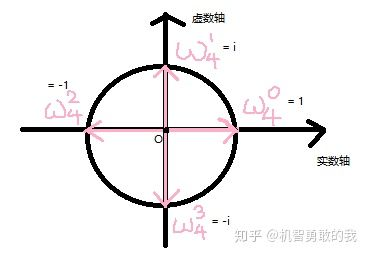
\includegraphics[width=0.7\textwidth]{docs/math/images/fft3.jpg} 
\caption{img}
\end{figure}

那么很容易发现当 $K = 4$ 的时候,相当于把单位圆等分 $K= 4$ 份。然后每一份按照极角编号。那么是不是(在 $K = 4$ 的时候)我们只要知道 $\omega_4^1$

(因为他的角度是相当于单位角度), 就能知道 $\omega_4^0, \omega_4^1, \omega_4^2, \omega_4^3$ 了呢?当然是这样的。。。

$\omega_4^0$ 恒等于 $1$,$\omega_4^2$ 的角度是 $\omega_4^0$ 的两倍,所以 $\omega_4^2 = (\omega_4^1)^2 = i^2=-1$, 依次以此类推。

因此,我们只要知道 $\omega_k^1$ ,就能求出 $\omega_k^n$。所以我们把 $\omega_k^1$ 称为单位复根,简写为 $\omega_k$

\subsection{FFT 的流程}

qwq 终于写到核心部分了,也就是,FFT 到底怎么来写呢?

\subsubsection{FFT 流程第一步之 DFT(共两步)}

FFT 之所以快,是因为他采用了分治的思想。

就 DFT(将系数表达转换成点值表达)来说,它分治的来求当当前的 $x=\omega_n^k$

的时候整个式子的值。他的分治思想体现在将多项式分为奇次项和偶次项处理。

对于一共 $8$ 项的多项式

$$
f(x0) = y_1 = a_0 + a_1x + a_2x^2+a_3x^3+a_4x^4+a_5x^5+a_6x^6+a_7x^7
$$

按照次数的奇偶来分成两组, 然后右边提出来一个 $x$

$$
f(x) = (a_0+a_2x^2+a_4x^4+a_6x^6) + (a_1x+a_3x^3+a_5x^5+a_7x^7)
$$

$$
f(x) = (a_0+a_2x^2+a_4x^4+a_6x^6) + x(a_1+a_3x^2+a_5x^4+a_7x^6)
$$

分别用奇偶次次项数建立新的方程

$$
G(x) = a_0+a_2x+a_4x^2+a_6x^3
$$

$$
H(x)=a_1+a_3x+a_5x^2+a_7x^3
$$

那么原来的 $f(x)$ 由新函数来表示 (是不是我们二分了一个多项式呢\textasciitilde{})

$$
F(x)=G(x^2) + x  \times  H(x^2)
$$

给函数带个帽子表示此时在进行的是 DFT 过程,把 x 代进去,即有

$$
DFT(f(\omega_n^k))=DFT(G((\omega_n^k)^2)) + \omega_n^k  \times  DFT(H((\omega_n^k)^2))
$$

!!!前方高能:

这个函数能处理的多项式长度只能是 $2^m(m \in N^ \times )$ , 否则在分治的时候左右不一样长,右边取不到系数了,程序没法进行。所以要在第一次 DFT 之前就把序列向上补成长度为 $2^m(m \in N^ \times )$(高次系数补 $0$)、最高项次数为 $n-1$ 的多项式。一定要预处理哦 qaq

然后我在代入值的时候,因为要代入 $n$ 个不同值,所以我们就代入 $\omega_n^0,\omega_n^1,\omega_n^2,\cdots, \omega_n^{n-1} (n=2^m(m \in N^ \times ))$

一共 $2^m$ 个不同值。

\begin{cppcode}
/*
 * 做 FFT
 *len 必须是 2^k 形式
 *on == 1 时是 DFT,on == -1 时是 IDFT
 */
void fft(Complex y[], int len, int on) {
  change(y, len);
  for (int h = 2; h <= len; h <<= 1) {
    Complex wn(cos(2 * PI / h), sin(on * 2 * PI / h));
    for (int j = 0; j < len; j += h) {
      Complex w(1, 0);
      for (int k = j; k < j + h / 2; k++) {
        Complex u = y[k];
        Complex t = w * y[k + h / 2];
        y[k] = u + t;
        y[k + h / 2] = u - t;
        w = w * wn;
      }
    }
  }
}
\end{cppcode}

但是这个算法还需要从 “分治” 的角度继续优化。我们每一次都会把整个多项式的奇数次项和偶数次项系数分开,一只分到只剩下一个系数。但是,这个递归的过程需要更多的内存。因此,我们可以先 “模仿递归” 把这些系数在原数组中 “拆分”,然后再 “倍增” 地去合并这些算出来的值。然而我们又要如何去拆分这些数呢?

设初始序列为 $\{x_0, x_1, x_2, x_3, x_4, x_5, x_6, x_7\}$

一次二分之后 $\{x_0, x_2, x_4, x_6\},\{x_1, x_3,x_5, x_7 \}$

两次二分之后 $\{x_0,x_4\} \{x_2, x_6\},\{x_1, x_3\},\{x_5, x_7 \}$

三次二分之后 $\{x_0\}\{x_4\}\{x_2\}\{x_6\}\{x_1\}\{x_3\}\{x_5\}\{x_7 \}$

有啥规律呢?其实就是原来的那个序列,每个数用二进制表示,然后把二进制翻转对称一下,就是最终那个位置的下标。比如 $x_1$ 是 001,翻转是 100,也就是 4,而且最后那个位置确实是 4,是不是很神奇啊\textbackslash{}\textasciitilde{}\textbackslash{}\textasciitilde{}\textasciitilde{}

这里附上代码

\begin{cppcode}
/*
 * 进行 FFT 和 IFFT 前的反置变换
 * 位置 i 和 i 的二进制反转后的位置互换
 *len 必须为 2 的幂
 */
void change(Complex y[], int len) {
  int i, j, k;
  for (int i = 1, j = len / 2; i < len - 1; i++) {
    if (i < j) swap(y[i], y[j]);
    // 交换互为小标反转的元素,i<j 保证交换一次
    // i 做正常的 + 1,j 做反转类型的 + 1,始终保持 i 和 j 是反转的
    k = len / 2;
    while (j >= k) {
      j = j - k;
      k = k / 2;
    }
    if (j < k) j += k;
  }
}
\end{cppcode}

\subsubsection{FFT 流程第二步之 IDFT(共两步)}

这一步 IDFT(傅里叶反变换)的作用我说的已经很清楚啦,就是把上一步获得的目标多项式的点值形式转换成系数形式。但是似乎并不简单呢(雾)。。。但是,我们把单位复根代入多项式之后,就是下面这个样子(矩阵表示方程组)

$$
 \begin{bmatrix}y[0] \\ y[1] \\ y[2] \\ y[3] \\ \dots \\ y[n-1] \end{bmatrix}
\begin{matrix}= \\ = \\ = \\ = \\ \\ = \end{matrix}
\begin{bmatrix}1 & 1 & 1 & 1 & \dots & 1 \\
1 & \omega_n^1 & \omega_n^2 & \omega_n^3 & \dots & \omega_n^{n-1} \\
1 & \omega_n^2 & \omega_n^4 & \omega_n^6 & \dots & \omega_n^{2(n-1)} \\
1 & \omega_n^3 & \omega_n^6 & \omega_n^9 & \dots & \omega_n^{3(n-1)} \\
\dots & \dots & \dots & \dots & \dots & \dots \\
1 & \omega_n^{n-1} & \omega_n^{2(n-1)} & \omega_n^{3(n-1)} & \dots & \omega_n^{(n-1)^2} \end{bmatrix}
\begin{bmatrix} a[0] \\ a[1] \\ a[2] \\ a[3] \\ \dots \\ a[n-1] \end{bmatrix} 
$$

而且现在我们已经得到最左边的结果了,中间的 $x$ 值在目标多项式的点值表示中也是一一对应的,所以,根据矩阵的基础知识,我们只要在式子两边左乘中间那个大矩阵的逆矩阵就行了。由于这个矩阵的元素非常特殊,他的逆矩阵也有特殊的性质,就是每一项取倒数,再除以 $n$,就能得到他的逆矩阵(这边根据的是单位原根的两个特殊性质推出来的,具体比较麻烦。如果想知道的话私我吧。)

如何改变我们的操作才能使计算的结果文原来的倒数呢?我们当然可以重新写一遍,但是这里有更简单的实现。这就要看我们求 “单位复根的过程了”:根据 “欧拉函数” $e^{i\pi}=-1$,我么可以得到 $e^{2\pi i}=1$。如果我要找到一个数,它的 $k$ 次方 $= 1$,那么这个数 $\omega[k]=e^{2\pi \frac{i}{k}}$(因为 $(e^{2\pi \frac{i}{k}})^k=e^{2\pi i}=1$)。而如果我要使这个数值变成$\frac{1}{\omega[k]}$ 也就是 $(\omega[k])^-1$,我们可以尝试着把

$π$ 取成 - 3.14159…,这样我们的计算结果就会变成原来的倒数,而其它的操作过程与 DFT 是完全相同的(这真是极好的)。我们可以定义一个函数,向里面掺一个参数 $1$ 或者是 $-1$,然后把它乘到 $π$ 的身上。传入 $1$ 就是 DFT,传入 $-1$ 就是 IDFT,十分的智能。

所以我们 fft 函数可以集 DFT 和 IDFT 于一身。见下

\begin{cppcode}
/*
 * 做 FFT
 *len 必须是 2^k 形式
 *on == 1 时是 DFT,on == -1 时是 IDFT
 */
void fft(Complex y[], int len, int on) {
  change(y, len);
  for (int h = 2; h <= len; h <<= 1) {                  // 模拟合并过程
    Complex wn(cos(2 * PI / h), sin(on * 2 * PI / h));  // 计算当前单位复根
    for (int j = 0; j < len; j += h) {
      Complex w(1, 0);  // 计算当前单位复根
      for (int k = j; k < j + h / 2; k++) {
        Complex u = y[k];
        Complex t = w * y[k + h / 2];
        y[k] = u + t;  // 这就是吧两部分分治的结果加起来
        y[k + h / 2] = u - t;
        // 后半个 “step” 中的ω一定和 “前半个” 中的成相反数
        //“红圈”上的点转一整圈“转回来”,转半圈正好转成相反数
        // 一个数相反数的平方与这个数自身的平方相等
        w = w * wn;
      }
    }
  }
  if (on == -1) {
    for (int i = 0; i < len; i++) {
      y[i].x /= len;
    }
  }
}
\end{cppcode}

好了现在附上全部代码(\href{http://acm.hdu.edu.cn/showproblem.php?pid=1402}{HDU 1402}),序言说过代码来自 kuangbin 的模板\sout{}\textasciitilde{} 来大家和我一起 Orz 一发

\begin{cppcode}
#include <cmath>
#include <cstdio>
#include <cstring>
#include <iostream>

using namespace std;

const double PI = acos(-1.0);
struct Complex {
  double x, y;
  Complex(double _x = 0.0, double _y = 0.0) {
    x = _x;
    y = _y;
  }
  Complex operator-(const Complex &b) const {
    return Complex(x - b.x, y - b.y);
  }
  Complex operator+(const Complex &b) const {
    return Complex(x + b.x, y + b.y);
  }
  Complex operator*(const Complex &b) const {
    return Complex(x * b.x - y * b.y, x * b.y + y * b.x);
  }
};
/*
 * 进行 FFT 和 IFFT 前的反置变换
 * 位置 i 和 i 的二进制反转后的位置互换
 *len 必须为 2 的幂
 */
void change(Complex y[], int len) {
  int i, j, k;
  for (int i = 1, j = len / 2; i < len - 1; i++) {
    if (i < j) swap(y[i], y[j]);
    // 交换互为小标反转的元素,i<j 保证交换一次
    // i 做正常的 + 1,j 做反转类型的 + 1,始终保持 i 和 j 是反转的
    k = len / 2;
    while (j >= k) {
      j = j - k;
      k = k / 2;
    }
    if (j < k) j += k;
  }
}
/*
 * 做 FFT
 *len 必须是 2^k 形式
 *on == 1 时是 DFT,on == -1 时是 IDFT
 */
void fft(Complex y[], int len, int on) {
  change(y, len);
  for (int h = 2; h <= len; h <<= 1) {
    Complex wn(cos(2 * PI / h), sin(on * 2 * PI / h));
    for (int j = 0; j < len; j += h) {
      Complex w(1, 0);
      for (int k = j; k < j + h / 2; k++) {
        Complex u = y[k];
        Complex t = w * y[k + h / 2];
        y[k] = u + t;
        y[k + h / 2] = u - t;
        w = w * wn;
      }
    }
  }
  if (on == -1) {
    for (int i = 0; i < len; i++) {
      y[i].x /= len;
    }
  }
}

const int MAXN = 200020;
Complex x1[MAXN], x2[MAXN];
char str1[MAXN / 2], str2[MAXN / 2];
int sum[MAXN];

int main() {
  while (scanf("%s%s", str1, str2) == 2) {
    int len1 = strlen(str1);
    int len2 = strlen(str2);
    int len = 1;
    while (len < len1 * 2 || len < len2 * 2) len <<= 1;
    for (int i = 0; i < len1; i++) x1[i] = Complex(str1[len1 - 1 - i] - '0', 0);
    for (int i = len1; i < len; i++) x1[i] = Complex(0, 0);
    for (int i = 0; i < len2; i++) x2[i] = Complex(str2[len2 - 1 - i] - '0', 0);
    for (int i = len2; i < len; i++) x2[i] = Complex(0, 0);
    fft(x1, len, 1);
    fft(x2, len, 1);
    for (int i = 0; i < len; i++) x1[i] = x1[i] * x2[i];
    fft(x1, len, -1);
    for (int i = 0; i < len; i++) sum[i] = int(x1[i].x + 0.5);
    for (int i = 0; i < len; i++) {
      sum[i + 1] += sum[i] / 10;
      sum[i] %= 10;
    }
    len = len1 + len2 - 1;
    while (sum[len] == 0 && len > 0) len--;
    for (int i = len; i >= 0; i--) printf("%c", sum[i] + '0');
    printf("\n");
  }
  return 0;
}
\end{cppcode}

至此,FFT 算是告一段落了。

但是,算竞选手可能像我一样有下面的疑问:

假如我要计算的多项式系数是别的具有特殊意义的整数,那么我通篇都在用浮点数运算,首先从时间上就会比整数运算慢,另外我最多只能用 long double 不能用 long long 类型,我能不能应用数论的变化从而避开浮点运算,达到 “更高更快更强 (・ω\&lt;) ” 呢?

\subsection{算竞选手看过来\textasciitilde{} NTT(数论优化的快速傅里叶变换)}

戳~  NTT 
